\subsubsection{Penguijan Deployment MQTT Client untuk Mengirim data Temperatur pada \textit{Clutser GCP}}

Pengujian ini mencakup pengujian dengan ID P32 hingga P39. Pada pengujian sistem ini, dilakukan proses \textit{remote deployment} MQTT pada \textit{cluster GCP} dengan cluster name "prod-cluster-example". Pengujian ini dilakukan untuk mensimulasikan node sebagai sebuah sensor temperatur yang akan mengirimkan data sensornya melalui mqtt client ke mqtt broker. Pengujian ini membuktikan  \textit{compatibility} dari sistem yang tidak terbatas pada IoT namun seluruh perangkat yang berbasis UNIX yang dapat menjalankan kubernetes. Proses \textit{remote deployment} dilakukan dengan menggunakan image gawrgare/mqtt-client yang telah dibuat dan di \textit{publish} pada \textit{dockerhub}. Script yang digunakan untuk membuat image docker dibuat dengan python serta akan mengirimkan data dalam interval 5 detik. \textit{Script} dapat dilihat pada gambar \ref{fig:pengujian-gcp-script-docker-images}

\begin{figure}[ht]
  \centering
  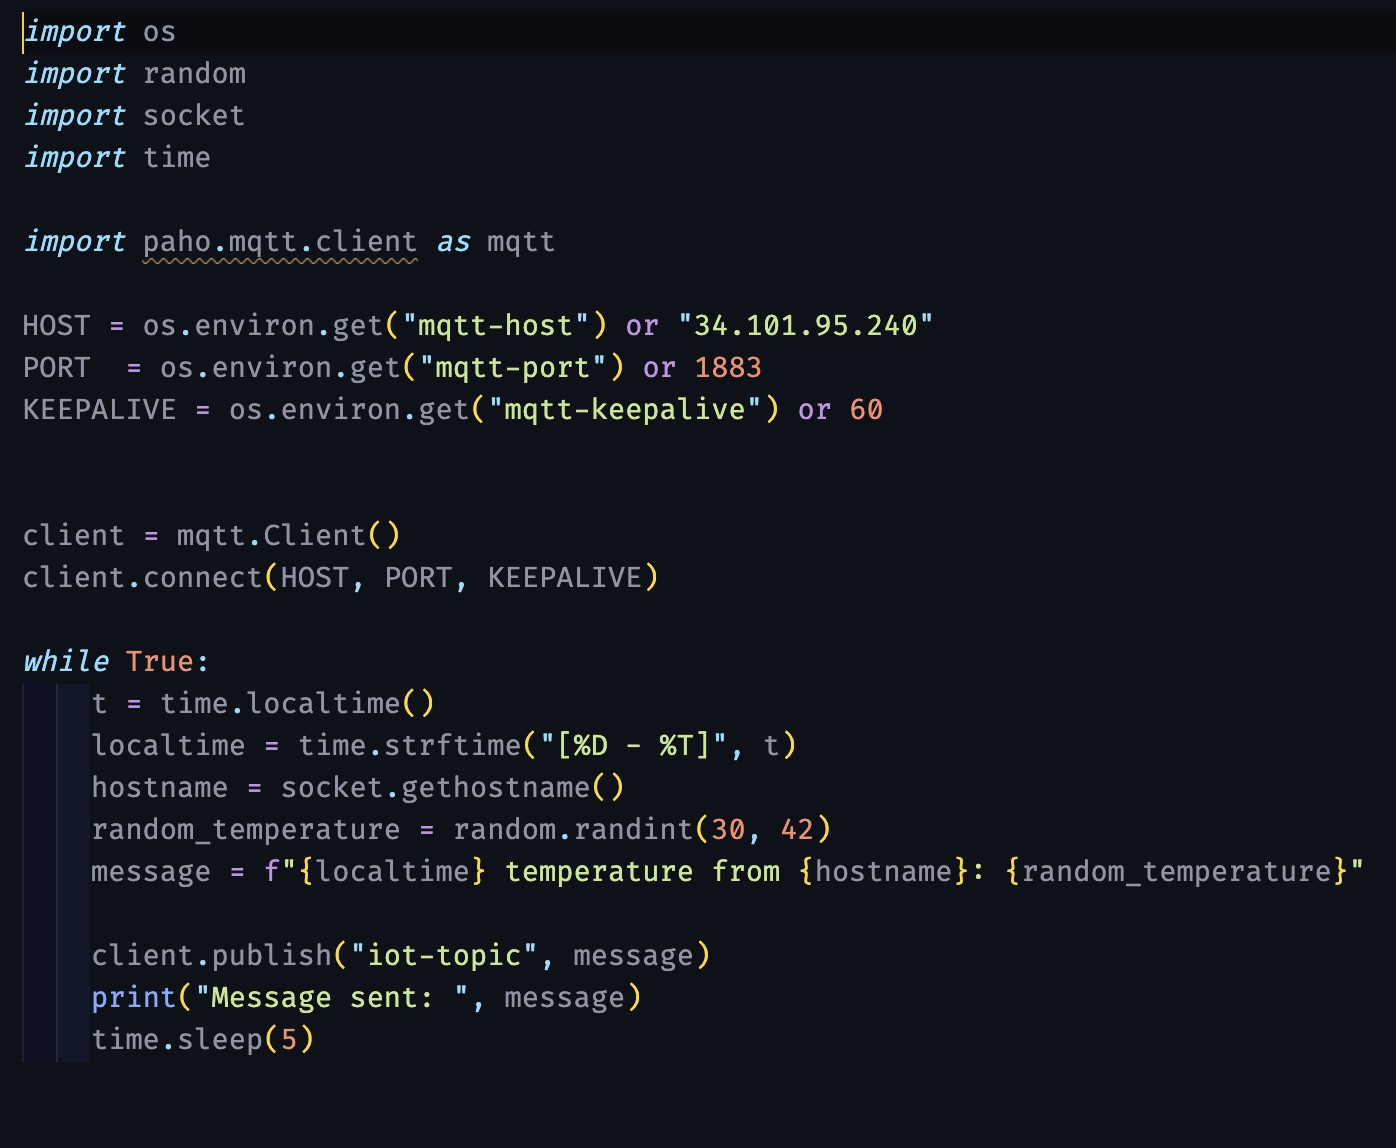
\includegraphics[width=0.8\textwidth]{resources/chapter-4/pengujian/pengujian-gcp-docker-image.jpg}
  \caption{Script MQTT Client untuk Docker Image gawrgare/mqtt-client}
  \label{fig:pengujian-gcp-script-docker-images}
\end{figure}

Pengujian dilakukan dengan mengikuti langkah langkah berikut:

\begin{enumerate}
  \item Melakukan setup mqtt-broker pada server yang memiliki IP 34.101.95.240.
  \item Membuat \textit{company} "test-semhas" dan nama cluster "prod-cluster-example". Hasil dapat dilihat pada lampiran \ref{fig:pengujian-sistem-gcp-01}
  \item Membuat \textit{user} dengan email "test@gmail.com", nama "test-user-semhas". Hasil dapat dilihat pada lampiran \ref{fig:pengujian-sistem-gcp-02}
  \item Login dengan menggunakan kredensial "test@gmail.com". Hasil dapat dilihat pada lampiran \ref{fig:pengujian-sistem-gcp-03}
  \item Mengunjungi halaman /devices lalu membuat \textit{device} "raspberrypi-pi-1" dan nama \textit{node} "master-cluster" serta memiliki label "sukses=aamiin". Hasil dapat dilihat pada lampiran \ref{fig:pengujian-sistem-gcp-04}
  \item Mengunjungi halaman /deployments lalu membuat \textit{deployment plan} untuk v1 dengan mengambil repository "gawrgare/mqtt-client" serta memiliki nama "mqtt-deployment". Hasil dapat dilihat pada lampiran \ref{fig:pengujian-sistem-gcp-05}
  \item Mengunjungi halaman /remote-deployment lalu melakukan \textit{deployment} dengan tipe "TARGET". Hasil dapat dilihat pada lampiran \ref{fig:pengujian-sistem-gcp-06}
  \item Setelah deployment berhasil dilakukan, hapus \textit{deployment} yang telah dibuat. Hasil dapat dilihat pada lampiran \ref{fig:pengujian-sistem-gcp-07}.
  \item Setelah deployment berhasil dibuat, jalankan kode untuk mengkonsumsi data dari mqtt-broker yang dikirimkan dari hasil deployment. Hasil dapat dilihat pada lampiran \ref{fig:pengujian-sistem-gcp-sukses-mqtt}
  \item Mengunjungi halaman /deployments lalu menghapus \textit{deployment plan} dengan nama "mqtt-deployment". Hasil dapat dilihat pada lampiran \ref{fig:pengujian-sistem-gcp-08}
  \item Mengunjungi halaman /deployments lalu menghapus \textit{deployment image} dengan nama "deploy-mqtt-client". Hasil dapat dilihat pada lampiran \ref{fig:pengujian-sistem-gcp-09}
\end{enumerate}

Setelah seluruh langkah dilakukan, pengujian dengan ID P32 hingga P39 berhasil diimplementasikan. Seluruh rekap pengujian dapat dilihat pada lampiran \ref{tab:pengujian-sistem-gcp}.